\documentclass[tikz,border=10pt]{standalone}
\usetikzlibrary{arrows.meta}

\definecolor{linkmain}{RGB}{68,108,148}
\definecolor{linksh}{RGB}{34,54,78}
\definecolor{linkhi}{RGB}{168,204,230}
\definecolor{basegray}{RGB}{150,150,150}
\definecolor{baselight}{RGB}{197,197,197}
\definecolor{basedark}{RGB}{100,100,100}
\definecolor{gripgray}{RGB}{95,95,100}

\begin{document}
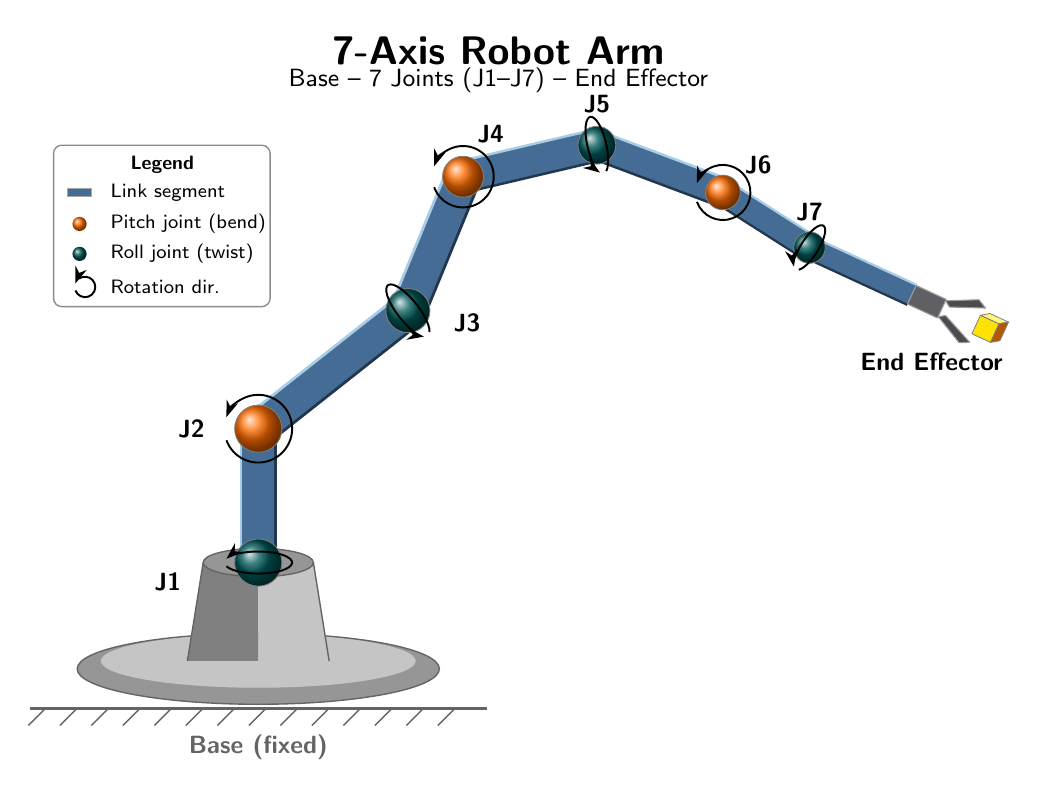
\begin{tikzpicture}[line join=round]

\tikzset{
  rotarrow/.style={-{Stealth[length=2.1mm,width=1.5mm]}, line width=0.7pt, black}
}

% ---------------------------------------------------------------
% coordinates : joint centers J1..J7 and end-effector anchor EE
% ---------------------------------------------------------------
\coordinate (J1) at (0,1.3);
\coordinate (J2) at (0,3.0);
\coordinate (J3) at (1.9,4.5);
\coordinate (J4) at (2.6,6.2);
\coordinate (J5) at (4.3,6.6);
\coordinate (J6) at (5.9,6.0);
\coordinate (J7) at (7.0,5.3);
\coordinate (EE) at (8.3,4.7);

% ---------------------------------------------------------------
% ground / fixed support hatching
% ---------------------------------------------------------------
\draw[line width=1pt, basedark] (-2.9,-0.55) -- (2.9,-0.55);
\foreach \x in {-2.7,-2.3,...,2.7}{
  \draw[basedark, line width=0.5pt] (\x,-0.55) -- ++(-0.22,-0.22);
}

% ---------------------------------------------------------------
% base pedestal (fixed to ground)
% ---------------------------------------------------------------
\filldraw[fill=basegray, draw=basedark, line width=0.5pt] (0,-0.05) ellipse (2.3 and 0.45);
\fill[baselight] (0,0.05) ellipse (2.0 and 0.34);
\fill[basegray!85!black] (-0.9,0.05) -- (0,0.05) -- (0,1.3) -- (-0.7,1.3) -- cycle;
\fill[baselight] (0,0.05) -- (0.9,0.05) -- (0.7,1.3) -- (0,1.3) -- cycle;
\draw[basedark, line width=0.5pt] (-0.9,0.05) -- (-0.7,1.3);
\draw[basedark, line width=0.5pt] (0.9,0.05) -- (0.7,1.3);
\filldraw[fill=basegray, draw=basedark, line width=0.5pt] (0,1.3) ellipse (0.7 and 0.18);
\node[font=\sffamily\bfseries\small, basedark] at (0,-1.05) {Base (fixed)};

% ---------------------------------------------------------------
% links L1..L7  (tapered rigid segments between joints)
% each link: filled quadrilateral + highlight edge + shadow edge
% ---------------------------------------------------------------
% L1 : J1 -> J2
\filldraw[fill=linkmain, draw=black!35, line width=0.3pt]
  (-0.220,1.300) -- (-0.220,3.000) -- (0.220,3.000) -- (0.220,1.300) -- cycle;
\draw[linkhi, line width=1pt] (-0.220,1.300) -- (-0.220,3.000);
\draw[linksh, line width=1pt] (0.220,1.300) -- (0.220,3.000);

% L2 : J2 -> J3
\filldraw[fill=linkmain, draw=black!35, line width=0.3pt]
  (-0.136,3.173) -- (1.764,4.673) -- (2.036,4.327) -- (0.136,2.827) -- cycle;
\draw[linkhi, line width=1pt] (-0.136,3.173) -- (1.764,4.673);
\draw[linksh, line width=1pt] (0.136,2.827) -- (2.036,4.327);

% L3 : J3 -> J4
\filldraw[fill=linkmain, draw=black!35, line width=0.3pt]
  (1.697,4.584) -- (2.397,6.284) -- (2.803,6.116) -- (2.103,4.416) -- cycle;
\draw[linkhi, line width=1pt] (1.697,4.584) -- (2.397,6.284);
\draw[linksh, line width=1pt] (2.103,4.416) -- (2.803,6.116);

% L4 : J4 -> J5
\filldraw[fill=linkmain, draw=black!35, line width=0.3pt]
  (2.554,6.395) -- (4.254,6.795) -- (4.346,6.405) -- (2.646,6.005) -- cycle;
\draw[linkhi, line width=0.9pt] (2.554,6.395) -- (4.254,6.795);
\draw[linksh, line width=0.9pt] (2.646,6.005) -- (4.346,6.405);

% L5 : J5 -> J6
\filldraw[fill=linkmain, draw=black!35, line width=0.3pt]
  (4.363,6.769) -- (5.963,6.169) -- (5.837,5.832) -- (4.237,6.432) -- cycle;
\draw[linkhi, line width=0.9pt] (4.363,6.769) -- (5.963,6.169);
\draw[linksh, line width=0.9pt] (4.237,6.432) -- (5.837,5.832);

% L6 : J6 -> J7
\filldraw[fill=linkmain, draw=black!35, line width=0.3pt]
  (5.986,6.135) -- (7.086,5.435) -- (6.914,5.165) -- (5.814,5.865) -- cycle;
\draw[linkhi, line width=0.8pt] (5.986,6.135) -- (7.086,5.435);
\draw[linksh, line width=0.8pt] (5.814,5.865) -- (6.914,5.165);

% L7 : J7 -> EE  (flange link into the end effector)
\filldraw[fill=linkmain, draw=black!35, line width=0.3pt]
  (7.059,5.427) -- (8.359,4.827) -- (8.241,4.573) -- (6.941,5.173) -- cycle;
\draw[linkhi, line width=0.8pt] (7.059,5.427) -- (8.359,4.827);
\draw[linksh, line width=0.8pt] (6.941,5.173) -- (8.241,4.573);

% ---------------------------------------------------------------
% joints J1..J7
%  - roll joints  (J1,J3,J5,J7) : teal spheres, elliptical "ring"
%    arrow aligned with the incoming link direction (twist about
%    the link's own axis)
%  - pitch joints (J2,J4,J6)    : orange spheres, circular arc
%    arrow drawn face-on (bend visible in the page plane)
% ---------------------------------------------------------------

% J1 - roll (base yaw, axis = link1 direction, vertical)
\shade[ball color=teal!70!black] (J1) circle (0.30);
\draw[black!50, line width=0.3pt] (J1) circle (0.30);
\begin{scope}[shift={(J1)}]
  \draw[rotarrow] (-0.4041,-0.0479) arc (200:520:0.43 and 0.14);
\end{scope}
\node[font=\sffamily\bfseries\small] at (-1.15,1.05) {J1};

% J2 - pitch (shoulder)
\shade[ball color=orange!85!red] (J2) circle (0.30);
\draw[black!50, line width=0.3pt] (J2) circle (0.30);
\draw[rotarrow] (-0.4041,2.8529) arc (200:520:0.43);
\node[font=\sffamily\bfseries\small] at (-0.85,3.00) {J2};

% J3 - roll (upper-arm roll, axis = link2 direction)
\shade[ball color=teal!70!black] (J3) circle (0.28);
\draw[black!50, line width=0.3pt] (J3) circle (0.28);
\begin{scope}[shift={(J3)}, rotate=128.29]
  \draw[rotarrow] (-0.3853,-0.0462) arc (200:520:0.41 and 0.135);
\end{scope}
\node[font=\sffamily\bfseries\small] at (2.65,4.35) {J3};

% J4 - pitch (elbow)
\shade[ball color=orange!85!red] (J4) circle (0.26);
\draw[black!50, line width=0.3pt] (J4) circle (0.26);
\draw[rotarrow] (2.2335,6.0666) arc (200:520:0.39);
\node[font=\sffamily\bfseries\small] at (2.95,6.75) {J4};

% J5 - roll (forearm roll, axis = link4 direction)
\shade[ball color=teal!70!black] (J5) circle (0.24);
\draw[black!50, line width=0.3pt] (J5) circle (0.24);
\begin{scope}[shift={(J5)}, rotate=103.24]
  \draw[rotarrow] (-0.3477,-0.0410) arc (200:520:0.37 and 0.12);
\end{scope}
\node[font=\sffamily\bfseries\small] at (4.30,7.12) {J5};

% J6 - pitch (wrist bend)
\shade[ball color=orange!85!red] (J6) circle (0.22);
\draw[black!50, line width=0.3pt] (J6) circle (0.22);
\draw[rotarrow] (5.5711,5.8803) arc (200:520:0.35);
\node[font=\sffamily\bfseries\small] at (6.35,6.35) {J6};

% J7 - roll (flange roll, axis = link6 direction)
\shade[ball color=teal!70!black] (J7) circle (0.20);
\draw[black!50, line width=0.3pt] (J7) circle (0.20);
\begin{scope}[shift={(J7)}, rotate=57.53]
  \draw[rotarrow] (-0.3101,-0.0376) arc (200:520:0.33 and 0.11);
\end{scope}
\node[font=\sffamily\bfseries\small] at (7.00,5.75) {J7};

% ---------------------------------------------------------------
% end effector : two-finger gripper holding a small workpiece,
% oriented along the J7->EE link direction (-24.775 deg)
% ---------------------------------------------------------------
\begin{scope}[shift={(EE)}, rotate=-24.775]
  % palm
  \filldraw[fill=gripgray, draw=black!40, line width=0.4pt]
    (0,-0.13) rectangle (0.42,0.13);
  % upper finger
  \filldraw[fill=gripgray!80!black, draw=black!40, line width=0.4pt]
    (0.42,0.11) -- (0.80,0.30) -- (0.92,0.24) -- (0.50,0.06) -- cycle;
  % lower finger
  \filldraw[fill=gripgray!80!black, draw=black!40, line width=0.4pt]
    (0.42,-0.11) -- (0.80,-0.30) -- (0.92,-0.24) -- (0.50,-0.06) -- cycle;
  % small workpiece (simple isometric-looking cube) held between the fingers
  \filldraw[fill=yellow!85!orange, draw=black!50, line width=0.3pt]
    (0.90,-0.13) rectangle (1.16,0.13);
  \filldraw[fill=yellow!50!white, draw=black!50, line width=0.3pt]
    (0.90,0.13) -- (1.16,0.13) -- (1.26,0.20) -- (1.00,0.20) -- cycle;
  \filldraw[fill=orange!70!black, draw=black!50, line width=0.3pt]
    (1.16,0.13) -- (1.26,0.20) -- (1.26,-0.06) -- (1.16,-0.13) -- cycle;
\end{scope}
\node[font=\sffamily\bfseries\small] at (8.55,3.85) {End Effector};

% ---------------------------------------------------------------
% title
% ---------------------------------------------------------------
\node[font=\sffamily\bfseries\Large] at (3.05,7.80) {7-Axis Robot Arm};
\node[font=\sffamily\small] at (3.05,7.42) {Base -- 7 Joints (J1--J7) -- End Effector};

% ---------------------------------------------------------------
% legend
% ---------------------------------------------------------------
\filldraw[fill=white, fill opacity=0.9, draw=black!45, line width=0.5pt, rounded corners=3pt]
  (-2.60,4.55) rectangle (0.15,6.60);
\node[font=\sffamily\bfseries\scriptsize] at (-1.22,6.35) {Legend};

\filldraw[fill=linkmain, draw=black!35, line width=0.3pt] (-2.42,5.95) rectangle (-2.12,6.05);
\node[font=\sffamily\scriptsize, anchor=west] at (-2.00,6.00) {Link segment};

\shade[ball color=orange!85!red] (-2.27,5.60) circle (0.09);
\node[font=\sffamily\scriptsize, anchor=west] at (-2.00,5.60) {Pitch joint (bend)};

\shade[ball color=teal!70!black] (-2.27,5.22) circle (0.09);
\node[font=\sffamily\scriptsize, anchor=west] at (-2.00,5.22) {Roll joint (twist)};

\draw[rotarrow] (-2.3222,4.7555) arc (200:520:0.13);
\node[font=\sffamily\scriptsize, anchor=west] at (-2.00,4.80) {Rotation dir.};

\end{tikzpicture}
\end{document}
